% se define una variable condicional para cada formato de salida
% a conditional variable is defined for each output format
\newif\ifPDF%
\newif\ifBNPDF%
\newif\ifEPUB%
\newif\ifHTML%
\newif\ifHTMLcinco%
\newif\ifJATS%
\newif\ifODT%

% \PDFtrue
 \BNPDFtrue
% \EPUBtrue
% \HTMLtrue
% \HTMLcincotrue
% \JATStrue
% \ODTtrue

% agregamos las referencias
% we added the references
\addbibresource{./files/gbTeXbib-CHARLAUBA2.bib}

% agregamos el glosario
% we added the glossary

\newglossaryentry{@glo200-latex}{
name         = {LaTeX},
description  = {es un sistema de composición de tipografía de alta calidad; incluye características diseñadas para la producción de documentación técnica y científica. LaTeX es la norma de facto para la comunicación y publicación de documentos científicos. Está disponible como software libre},
text         = {LaTeX},
}
\newglossaryentry{@glo201-ceheal}{
type = \acronymtype,
name         = {CEHEAL},
description  = {Centro de Estudios de Historia Económica Latinoamericana y Argentina},
first        = {Centro de Estudios de Historia Económica Latinoamericana y Argentina (CEHEAL)},
text         = {CEHEAL},
}

% los metadatos son opcionales en el PDF a diferencia del resto que es obligatorio y se cargan automáticamente
% the metadata is optional in the PDF, unlike the rest which is mandatory and loaded automatically
\ifODT
\usepackage[unicode,hyperindex=true]{hyperref}
\else
	\ifPDF
	% control de inconsistencias de principio y fin de linea
	% inconsistency control of start and end of line (homeoarchy)
	\usepackage[hyphenation,homeoarchy,draft,homeoarchywordcolor=yellow,homeoarchycharcolor=yellow]{impnattypo}
	\usepackage[allcolors=magenta,colorlinks]{hyperref}
	\usepackage{hyperxmp}
	\hypersetup{
pdfauthor={Alberto Moyano},
pdfsubtitle={a},
pdfauthortitle={a},
pdfdate={2024-22},
pdfcopyright={GNU General Public License},
pdflicenseurl={https://es.wikipedia.org/wiki/GNU_General_Public_License},
pdftype={Text},
pdfpubtype={book},
pdfpagerange={0},
pdfisbn={0},
pdflang={es-ES},
pdfmetalang={es},
pdfrendition={default},
pdfx={pdf/A},
pdfformato={15.5x23cm},
pdftitle={a},
pdfcreator={gbTeXpublisher},
pdfproducer={Ecosistema de LaTeX},
unicode=true,
bookmarks=true,
pdfdisplaydoctitle=true,
pdfnewwindow=true
}

	\else
		\ifBNPDF
		\usepackage[cam,width=18truecm,height=25.5truecm,center]{crop}
		\usepackage[hidelinks]{hyperref}
		\usepackage{hyperxmp}
		\hypersetup{
pdfauthor={Alberto Moyano},
pdfsubtitle={a},
pdfauthortitle={a},
pdfdate={2024-22},
pdfcopyright={GNU General Public License},
pdflicenseurl={https://es.wikipedia.org/wiki/GNU_General_Public_License},
pdftype={Text},
pdfpubtype={book},
pdfpagerange={0},
pdfisbn={0},
pdflang={es-ES},
pdfmetalang={es},
pdfrendition={default},
pdfx={pdf/A},
pdfformato={15.5x23cm},
pdftitle={a},
pdfcreator={gbTeXpublisher},
pdfproducer={Ecosistema de LaTeX},
unicode=true,
bookmarks=true,
pdfdisplaydoctitle=true,
pdfnewwindow=true
}

		\else
			\ifEPUB
			\usepackage[hyperindex=true,allcolors=magenta,colorlinks]{hyperref}
			\fi
		\fi
	\fi
\fi

\begin{document}
\frontmatter

\ifEPUB%
	\ifdefined\HCode
	\phantomsection
	\addcontentsline{toc}{section}{Portada}
	\coverimage{./media/cover.png}
	\clearpage
	\fi
\fi

\ifPDF
% página 1
\newpage
\thispagestyle{empty}
{\textcolor{white}{.}}

% página 2
\newpage
\thispagestyle{empty}
{\textcolor{white}{.}}

% página 3
\newpage
\thispagestyle{empty}
{\textcolor{white}{.}}

\vspace{30mm}

\begin{center}
	\LARGE{III Jornada Latinoamericana\\ de Estudios Editoriales}
\end{center}

% página 4
\newpage
\thispagestyle{empty}
{\textcolor{white}{.}}

% página 5
\newpage
\thispagestyle{empty}
\begin{center}%,draft
{\sc\large{alberto moyano}}\\ %compiladoras
\end{center}

\vspace{30mm}

\begin{center}
\LARGE{III Jornada Latinoamericana\\ de Estudios Editoriales}\\\vspace{10mm}

\Large{Por la educación pública y el derecho\\ a la enseñanza universitaria}
\end{center}

\vfill

\begin{figure}[b]
\centering

\includegraphics[width=30mm]{./media/logo-LaTeX.png}
\end{figure}

% página 6
\newpage
\thispagestyle{empty}
\begin{figure}[t]
\centering
\vspace{-10mm}

\includegraphics[width=20mm]{./media/logo-GNU.png}\\
%\sc{colección...}%
\end{figure}

\noindent autor \\
\noindent título. 1a ed. Buenos Aires: 2024.\\
\noindent 000 p.; 15.5x23 cm. ISBN 978-950-793-000-0 \\
\noindent 1. \\
\noindent CDD .\\
\noindent Fecha de catalogación: 00/00/2024 \\
\noindent \textcopyright~20xx, autor \\
\noindent \textcopyright~20xx, Ediciones Imago Mundi\\
\noindent Imagen de tapa: .\\
\noindent Hecho el depósito que marca la ley 11.723\\
\noindent Impreso en Argentina, tirada de esta edición: 000 ejemplares\\

\vfill

\noindent Ninguna parte de esta publicación, incluido el diseño de cubierta, puede ser reproducida, almacenada o transmitida de manera alguna ni por ningún medio, ya sea eléctrico, químico, mecánico, óptico, de grabación o de fotocopia, sin permiso previo por escrito del editor. Este libro se terminó de imprimir en el mes de xxxx de 2024 en San Carlos Impresiones, Virrey Liniers 2203, Ciudad Autónoma de Buenos Aires, República Argentina.

\else
	\ifBNPDF
	% página 1
\newpage
\thispagestyle{empty}
{\textcolor{white}{.}}

% página 2
\newpage
\thispagestyle{empty}
{\textcolor{white}{.}}

% página 3
\newpage
\thispagestyle{empty}
{\textcolor{white}{.}}

\vspace{30mm}

\begin{center}
	\LARGE{III Jornada Latinoamericana\\ de Estudios Editoriales}
\end{center}

% página 4
\newpage
\thispagestyle{empty}
{\textcolor{white}{.}}

% página 5
\newpage
\thispagestyle{empty}
\begin{center}%,draft
{\sc\large{alberto moyano}}\\ %compiladoras
\end{center}

\vspace{30mm}

\begin{center}
\LARGE{III Jornada Latinoamericana\\ de Estudios Editoriales}\\\vspace{10mm}

\Large{Por la educación pública y el derecho\\ a la enseñanza universitaria}
\end{center}

\vfill

\begin{figure}[b]
\centering

\includegraphics[width=30mm]{./media/logo-LaTeX.png}
\end{figure}

% página 6
\newpage
\thispagestyle{empty}
\begin{figure}[t]
\centering
\vspace{-10mm}

\includegraphics[width=20mm]{./media/logo-GNU.png}\\
%\sc{colección...}%
\end{figure}

\noindent autor \\
\noindent título. 1a ed. Buenos Aires: 2024.\\
\noindent 000 p.; 15.5x23 cm. ISBN 978-950-793-000-0 \\
\noindent 1. \\
\noindent CDD .\\
\noindent Fecha de catalogación: 00/00/2024 \\
\noindent \textcopyright~20xx, autor \\
\noindent \textcopyright~20xx, Ediciones Imago Mundi\\
\noindent Imagen de tapa: .\\
\noindent Hecho el depósito que marca la ley 11.723\\
\noindent Impreso en Argentina, tirada de esta edición: 000 ejemplares\\

\vfill

\noindent Ninguna parte de esta publicación, incluido el diseño de cubierta, puede ser reproducida, almacenada o transmitida de manera alguna ni por ningún medio, ya sea eléctrico, químico, mecánico, óptico, de grabación o de fotocopia, sin permiso previo por escrito del editor. Este libro se terminó de imprimir en el mes de xxxx de 2024 en San Carlos Impresiones, Virrey Liniers 2203, Ciudad Autónoma de Buenos Aires, República Argentina.

	\fi
\fi

\ifPDF
\Author{Sumario}
\else
	\ifBNPDF
	\Author{Sumario}
	\fi
\fi

\tableofcontents

\chapter{Frontmatter}

La formación2                                           de \gls{@glo202-joseingenieros}\index[onomastico]{Ingenieros, José} fue universitaria y a diferencia del lugar tradicional del docente y del académico, su obra adquirió una marcada proyección política logrando complejas derivaciones que no son fácilmente encuadrables en un solo espacio partidario, si bien sus ideas estuvieron ligadas mayoritariamente a la tradición de izquierda socialista.2








Su vida y su obra habilitaron una diversidad de relecturas, de articulaciones políticas y de reapropiaciones teóricas. Esta particularidad caracterizó a \gls{@glo195-coas} y también a muchos de sus compañeros de militancia como el mexicano José Vasconcelos\index[onomastico]{Vasconcelos, José} o los argentinos Leopoldo Lugones\index[onomastico]{Lugones, Leopoldo} y Manuel Ugarte\index[onomastico]{Ugarte, Manuel} \parencite{@2762-MONSIVAIS1994}.

\mainmatter

\chapter{MainmatterA}

\section{SecciónA}

Esta obra colectiva da continuidad a uno de los programas centrales impulsados por el \gls{@glo201-ceheal} desde su creación en 2019: el estudio de las ideas y del pensamiento económico en su vínculo con la implementación de políticas económicas.\footnote{Una nota a pie de página.}

La secuencia de Fibonacci es una serie matemática en la cual cada número es la suma de los dos anteriores, comenzando generalmente con 0 y 1. La fórmula general para la secuencia de Fibonacci se puede expresar matemáticamente de la siguiente manera:

$$F(n) = F(n-1) + F(n-2)$$

\ifPDF
\froufrou
\else
	\ifBNPDF
	\froufrou
	\else
		\ifODT
		\begin{center} * * * \end{center}
		\fi
	\fi
\fi

\section{SecciónAA}

Esta obra colectiva da continuidad a uno de los programas centrales impulsados por el \gls{@glo201-ceheal} desde su creación en 2019: el estudio de las ideas y del pensamiento económico en su vínculo con la implementación de políticas económicas\index[concepto]{Políticas económicas para la sociedad} \parencite{@2761-RODRIGUEZRIVA2019}.

\chapter{MainmatterB}

\section{SecciónB}

Esta obra colectiva da continuidad a uno de los programas centrales impulsados por el \gls{@glo201-ceheal} desde su creación en 2019: el estudio de las ideas y del pensamiento económico en su vínculo con la implementación de políticas económicas.

\ifPDF%
\begin{figure}[!ht]
\centering
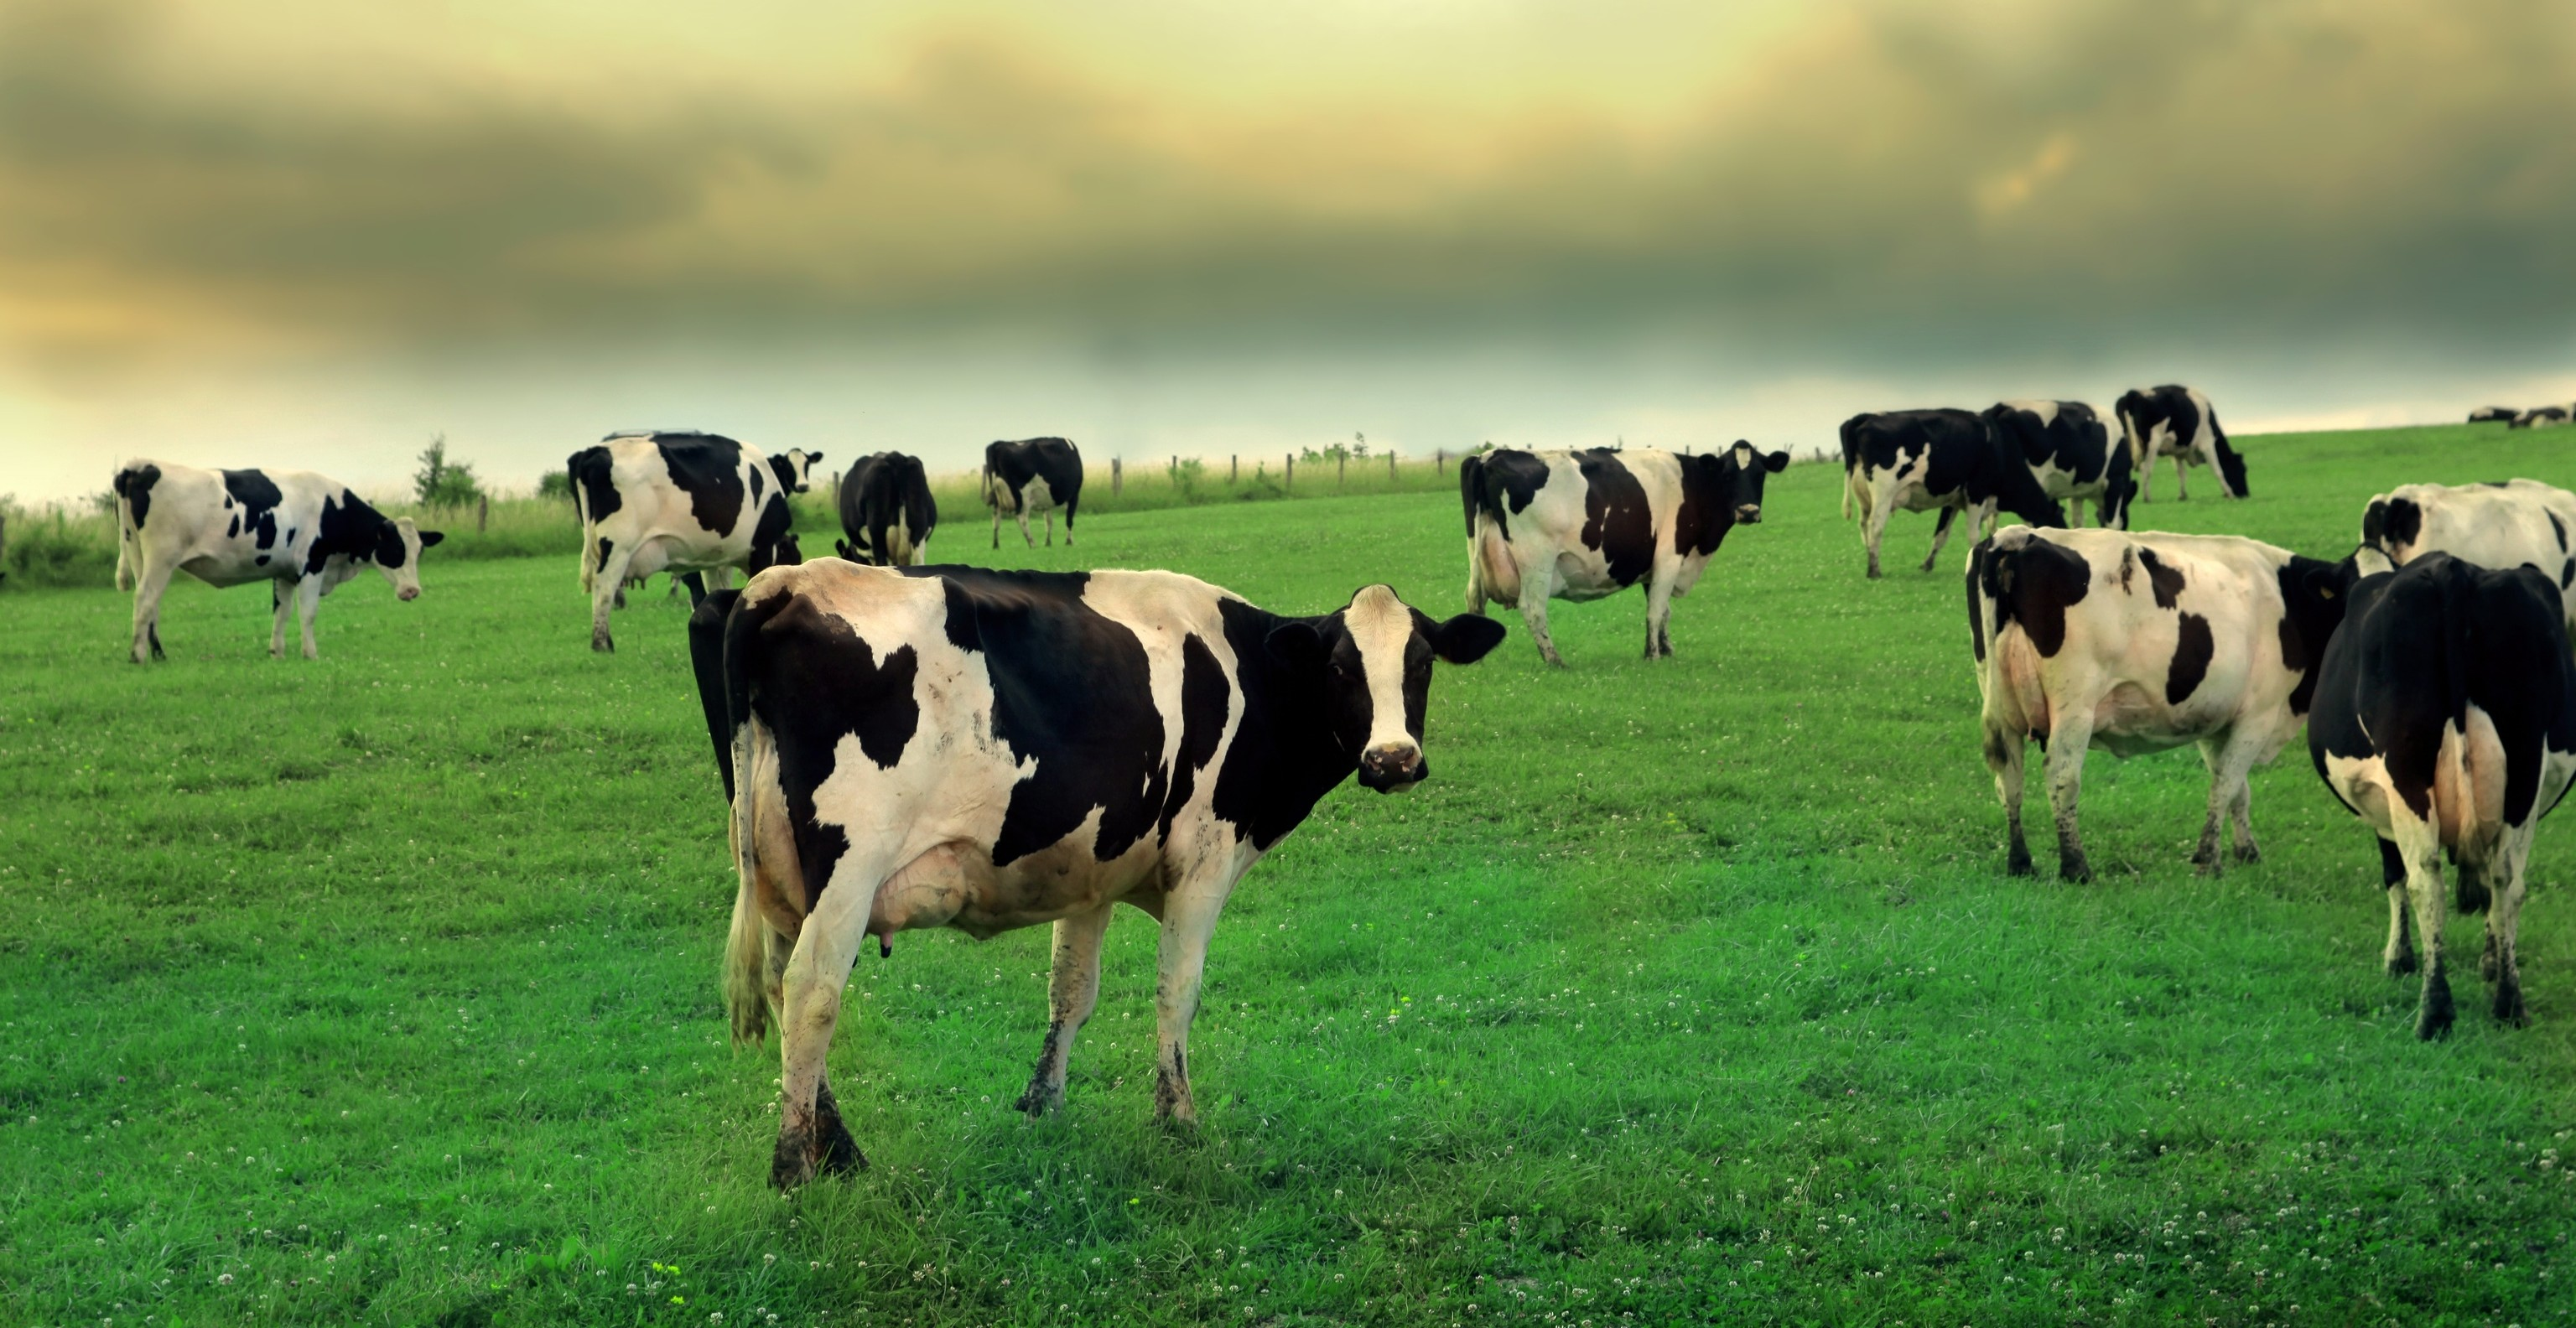
\includegraphics[width=\textwidth]{./media/imagen1.jpg}
\caption{Este es el epígrafe de la figura a color.}
\end{figure}
\else
	\ifBNPDF%
	\begin{figure}[!ht]
	\centering
	
\includegraphics[width=\textwidth]{./media/bn-imagen1.png}
	\caption{Este es el epígrafe de la figura en escala de grises.}
	\end{figure}
	\else
		\ifODT%
		\begin{figure}[!ht]
		\centering
		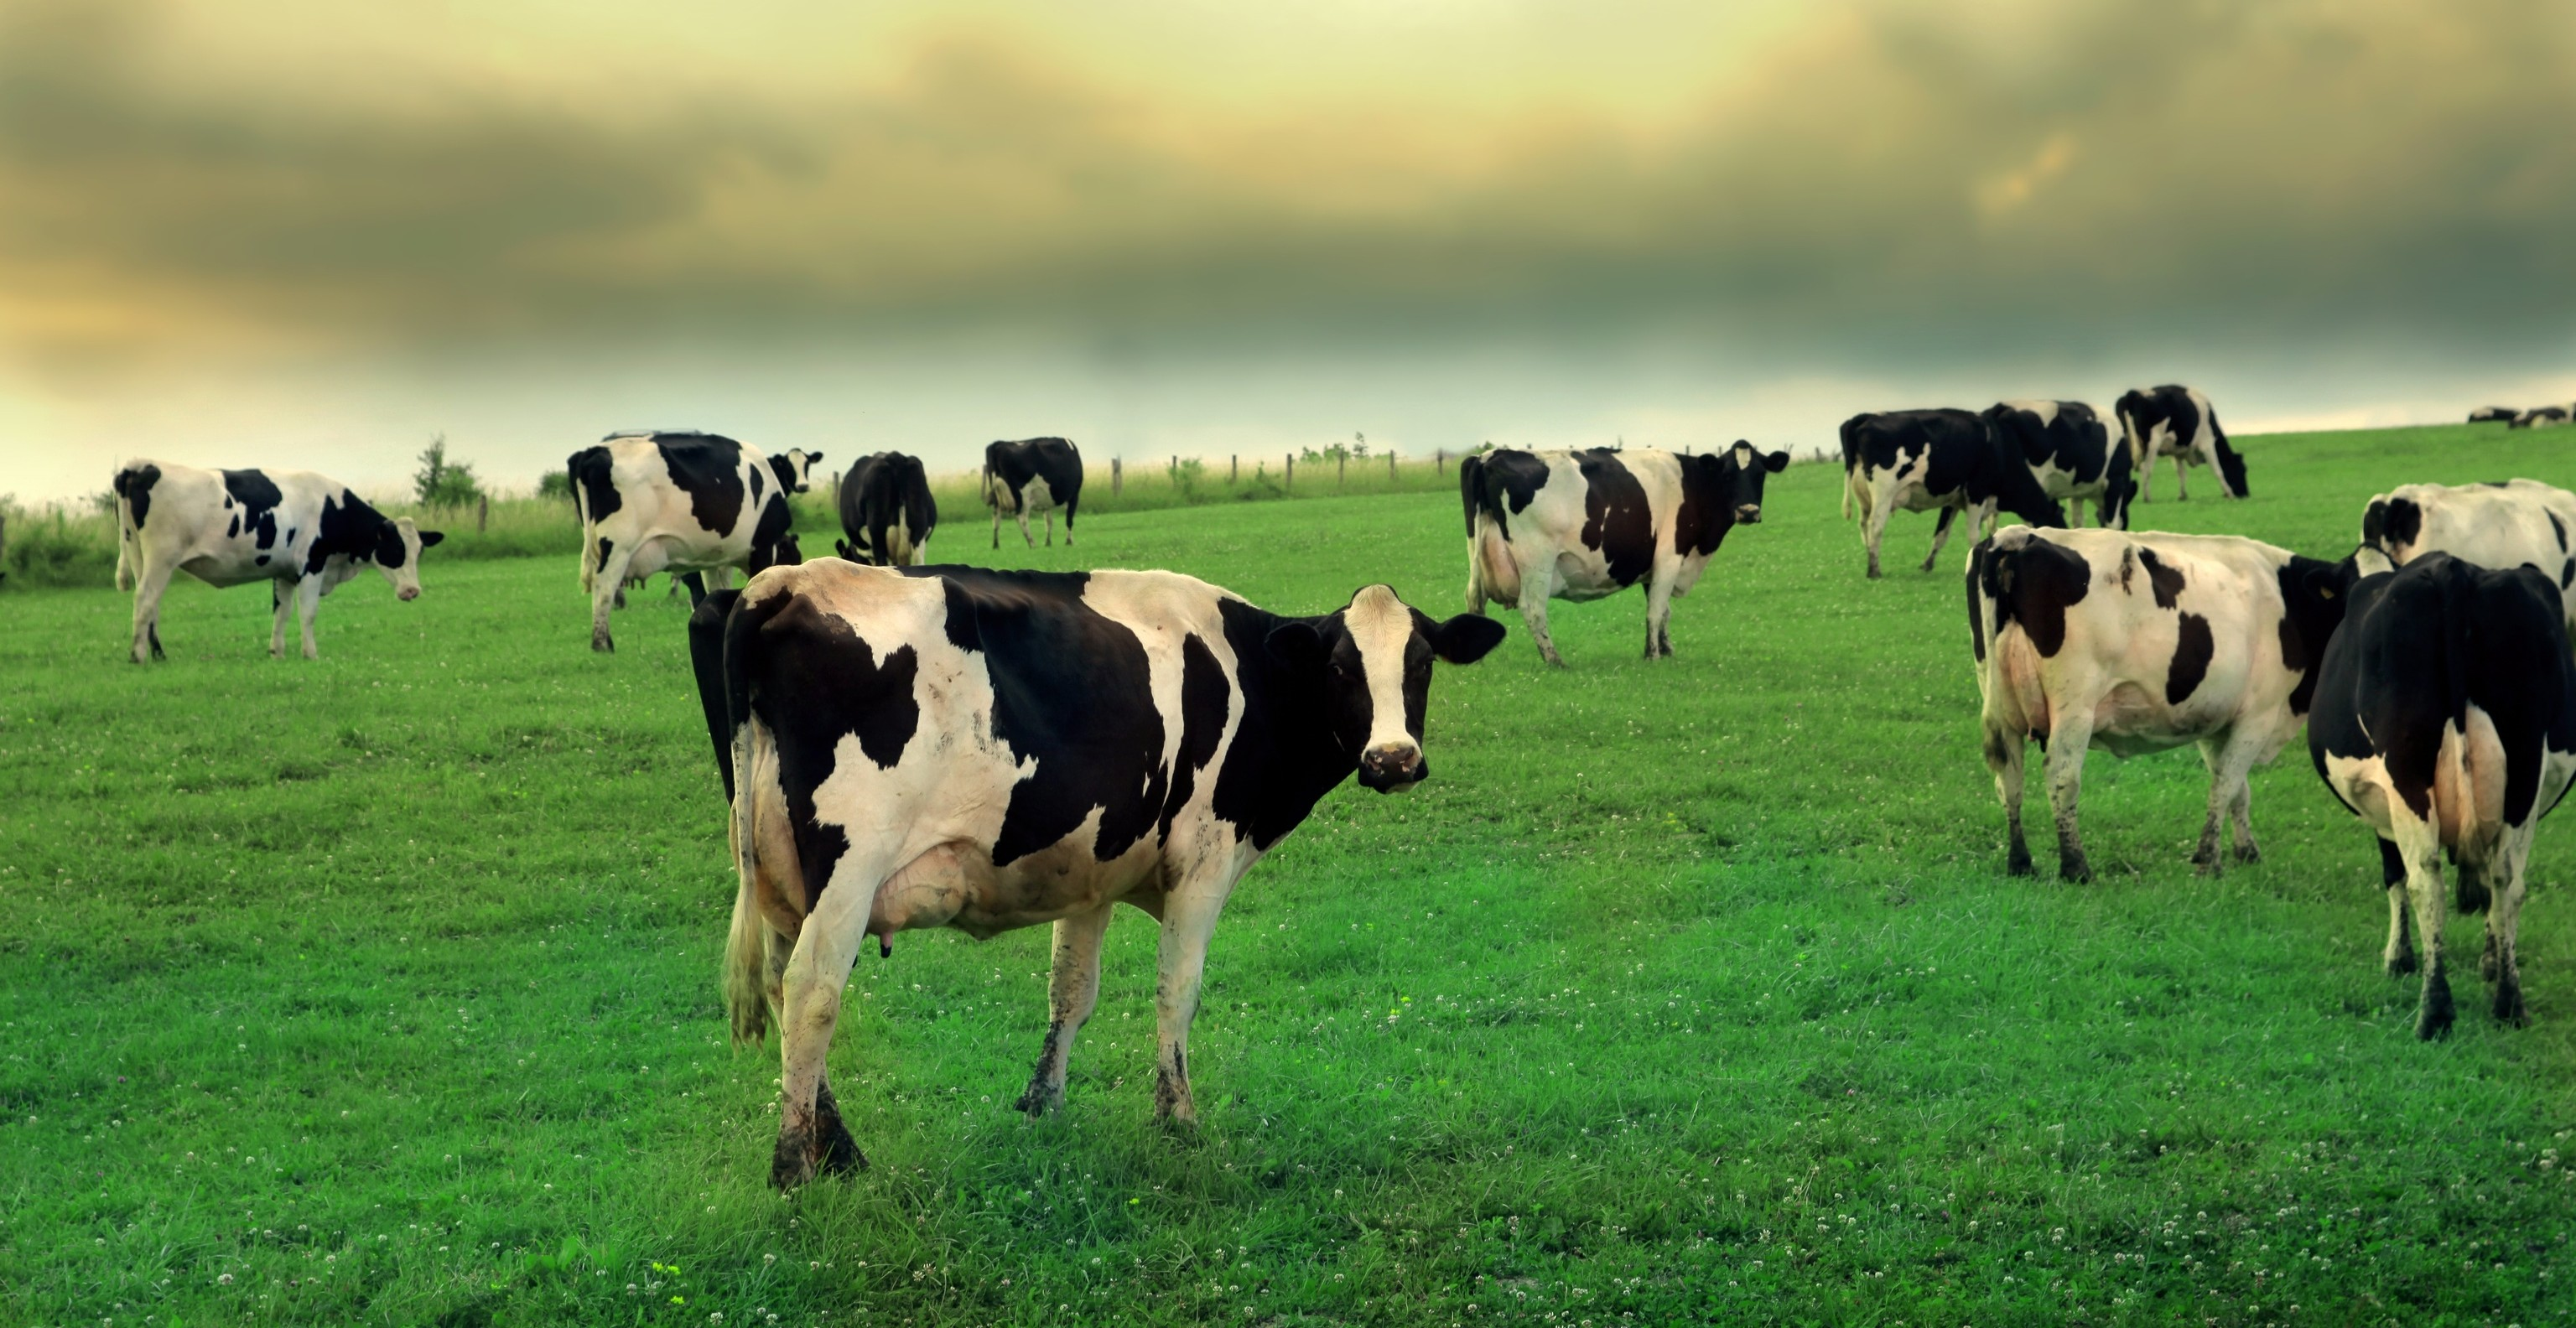
\includegraphics[width=\textwidth]{./media/imagen1.jpg}
		\caption{Este es el epígrafe de la figura a color.}
		\end{figure}
		\else
			\ifEPUB
			\begin{figure}[!ht]
			\centering
			
\includegraphics[width=\textwidth]{./media/bn-imagen1.png}
			\caption{Este es el epígrafe de la figura a color.}
			\end{figure}
			\fi
		\fi
	\fi
\fi

\section{SecciónBB}

Esta obra colectiva da continuidad a uno de los programas centrales impulsados por el \gls{@glo201-ceheal} desde su creación en 2019: el estudio de las ideas y del pensamiento económico en su vínculo con la implementación de políticas económicas.\footnote{Nota a pie en una sección del segundo capítulo.}

\backmatter

%Condicional para llevar todas las notas a pie al final del libro como un capítulo.
%Conditional to move all the footnotes to the end of the book as a chapter
\ifEPUB
\begingroup
\parindent 0pt
\parskip 2ex
\def\enotesize{\normalsize}
\theendnotes
\endgroup
\fi

\ifPDF
\printnoidxglossary[type=\acronymtype,title={Índice de siglas}]
\printnoidxglossary[title={Glosario de términos}]
\printbibliography[heading=none,heading=bibintoc]
\else
	\ifBNPDF
	\printnoidxglossary[type=\acronymtype,title={Índice de siglas}]
	\printnoidxglossary[title={Glosario de términos}]
	\printbibliography[heading=none,heading=bibintoc]
	\else
		\ifODT
		\printnoidxglossary[type=\acronymtype,title={Índice de siglas}]
		\printnoidxglossary[title={Glosario de términos}]
		\printbibliography[heading=none,heading=bibintoc]
		\else
			\ifEPUB
			\printnoidxglossary[type=\acronymtype,title={Índice de siglas}]
			\printnoidxglossary[title={Glosario de términos}]
			\chapter{Bibliografía}
			\printbibliography[heading=none]
			\fi
		\fi
	\fi
\fi





\ifPDF
\printindex[names]
\printindex[concepto]
\printindex[onomastico]
\Author{Índice de autoras y autores}
\else
	\ifBNPDF
	\printindex[names]
	\printindex[concepto]
	\printindex[onomastico]
	\Author{Índice de autoras y autores}
% \else
% 	\ifEPUB
% 	\printindex[names]
% 	\printindex[concepto]
% 	\printindex[onomastico]
% 	\fi
	\fi
\fi

\chapter{Colofón}

La composición tipográfica de este libro se realizó utilizando el lenguaje \gls{@glo200-latex} y el software gbTeXpublisher.

Las familias tipográficas utilizadas dentro del libro son: IBM Plex, una superfamilia de tipografía abierta, diseñada y desarrollada conceptualmente por Mike Abbink en IBM con colaboración de Bold Monday y Libertinus, bifurcación de la fuente Linux Libertine, diseñada para el texto del cuerpo y la lectura extendida.

\ifPDF
\newpage
\thispagestyle{empty}
{\textcolor{white}{.}}
\else
	\ifBNPDF
	\newpage
	\thispagestyle{empty}
	{\textcolor{white}{.}}
	\fi
\fi

\end{document}



